\begin{frame}
\frametitle{Первый процесс}
\begin{itemize}
    \item<1->Ядро ОС настроило прерывания, аллокаторы, планировщик. Что дальше?
    \begin{itemize}
        \item<2->мы должны запустить первый процесс и первое приложение!
        \item<3->например, Linux проверяет файлы: /sbin/init, /etc/init,
             /bin/init и /bin/sh.
    \end{itemize}
\end{itemize}
\end{frame}

\begin{frame}
\frametitle{Исполняемые файлы}
\begin{itemize}
    \item<1->Существует множество форматов исполняемых файлов:
    \begin{itemize}
        \item<2->ELF, a.out, PE, COM, Mach-O;
        \item<3->скрипты, начинающиеся с \#! (sha-bang).
    \end{itemize}
\end{itemize}
\end{frame}

\begin{frame}
\frametitle{Заголовок исполняемого файла}
\begin{itemize}
    \item<1->Заголовок:
    \begin{itemize}
        \item<2->magic number/string - позволяет быстро определить формат файла;
        \item<3->различного рода флаги и параметры:
        \begin{itemize}
            \item<4->версия формата исполняемого файла;
            \item<5->архитектура;
            \item<6->ссылки на другие части файла.
        \end{itemize}
    \end{itemize}
\end{itemize}
\end{frame}

\begin{frame}[fragile]
\frametitle{Заголовок ELF файла}
\begin{lstlisting}
    struct elf64_hdr {
        uint8_t e_ident[16];
        uint16_t e_type;
        uint16_t e_machine;
        uint32_t e_version;
        uint64_t e_entry;
        uint64_t e_phoff;
        uint64_t e_shoff;
        uint32_t e_flags;
        uint16_t e_ehsize;
        uint16_t e_phentsize;
        uint16_t e_phnum;
        uint16_t e_shentsize;
        uint16_t e_shnum;
        uint16_t e_shstrndx;
    } __attribute__((packed));
\end{lstlisting}
\end{frame}

\begin{frame}
\frametitle{Точка входа}
\begin{itemize}
    \item<1->У любой программы есть первая инструкция - точка входа:
    \begin{itemize}
        \item<2->формат исполняемого файла явно или не явно указывает адрес
             первой инструкции;
        \item<3->ОС после загрузки исполняемого файла передает управление первой
             инструкции;
        \item<4->обычно передача управления сопровождается понижением уровня
             привилегий кода (переходом в userspace).
    \end{itemize}
\end{itemize}
\end{frame}

\begin{frame}[fragile]
\frametitle{Заголовок ELF файла}
\begin{lstlisting}
    struct elf64_hdr {
        uint8_t e_ident[16];
        uint16_t e_type;
        uint16_t e_machine;
        uint32_t e_version;

        /* Logical address of the first instruction */
        uint64_t e_entry;

        uint64_t e_phoff;
        uint64_t e_shoff;
        uint32_t e_flags;
        uint16_t e_ehsize;
        uint16_t e_phentsize;
        uint16_t e_phnum;
        uint16_t e_shentsize;
        uint16_t e_shnum;
        uint16_t e_shstrndx;
    } __attribute__((packed));
\end{lstlisting}
\end{frame}

\begin{frame}
\frametitle{Описание адресного пространства}
\begin{itemize}
    \item<1->Формат исполняемого файла описывает логическое адресное
         пространство:
    \begin{itemize}
        \item<2->какие участки логического адресного пространства нужны
             и для чего;
        \item<3->где в памяти процесса должны располагаться код и данные;
        \item<4->где в исполняемом файле хранятся код и данные.
    \end{itemize}
\end{itemize}
\end{frame}

\begin{frame}
\frametitle{Типичное адресное пространство}
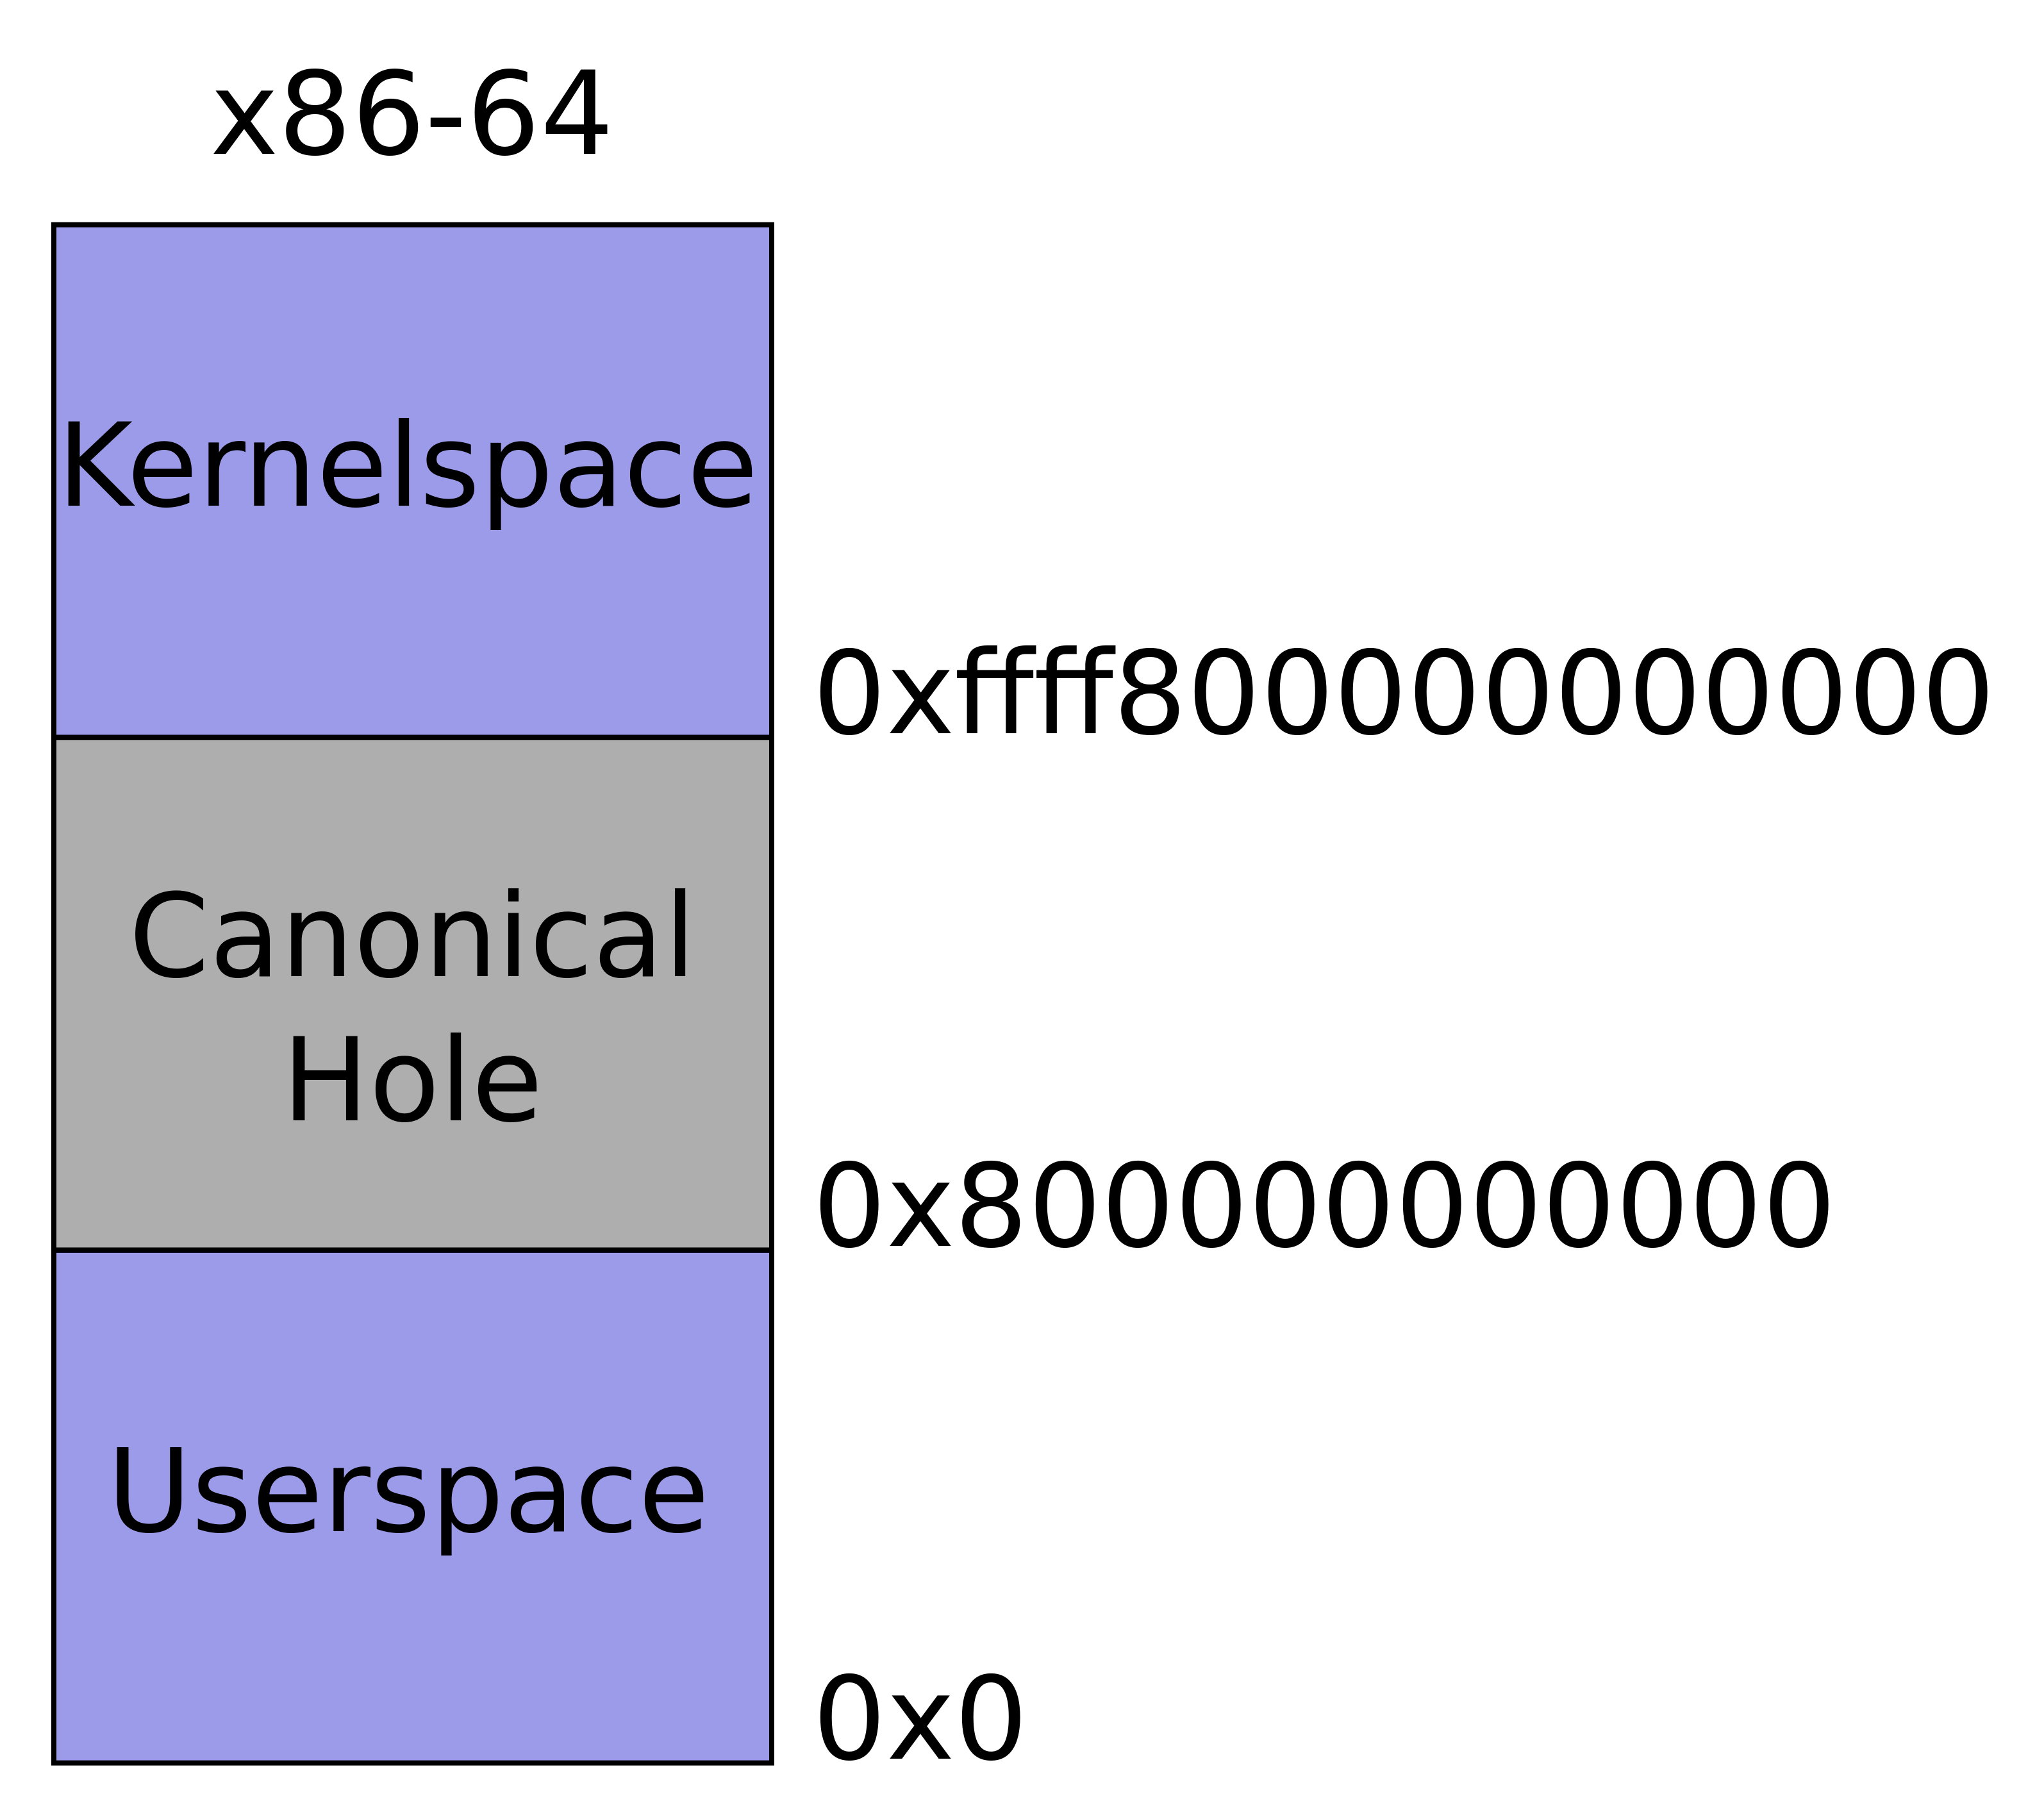
\includegraphics[height=.6\textheight]{amd64}
\end{frame}

\begin{frame}
\frametitle{Типичное адресное пространство}
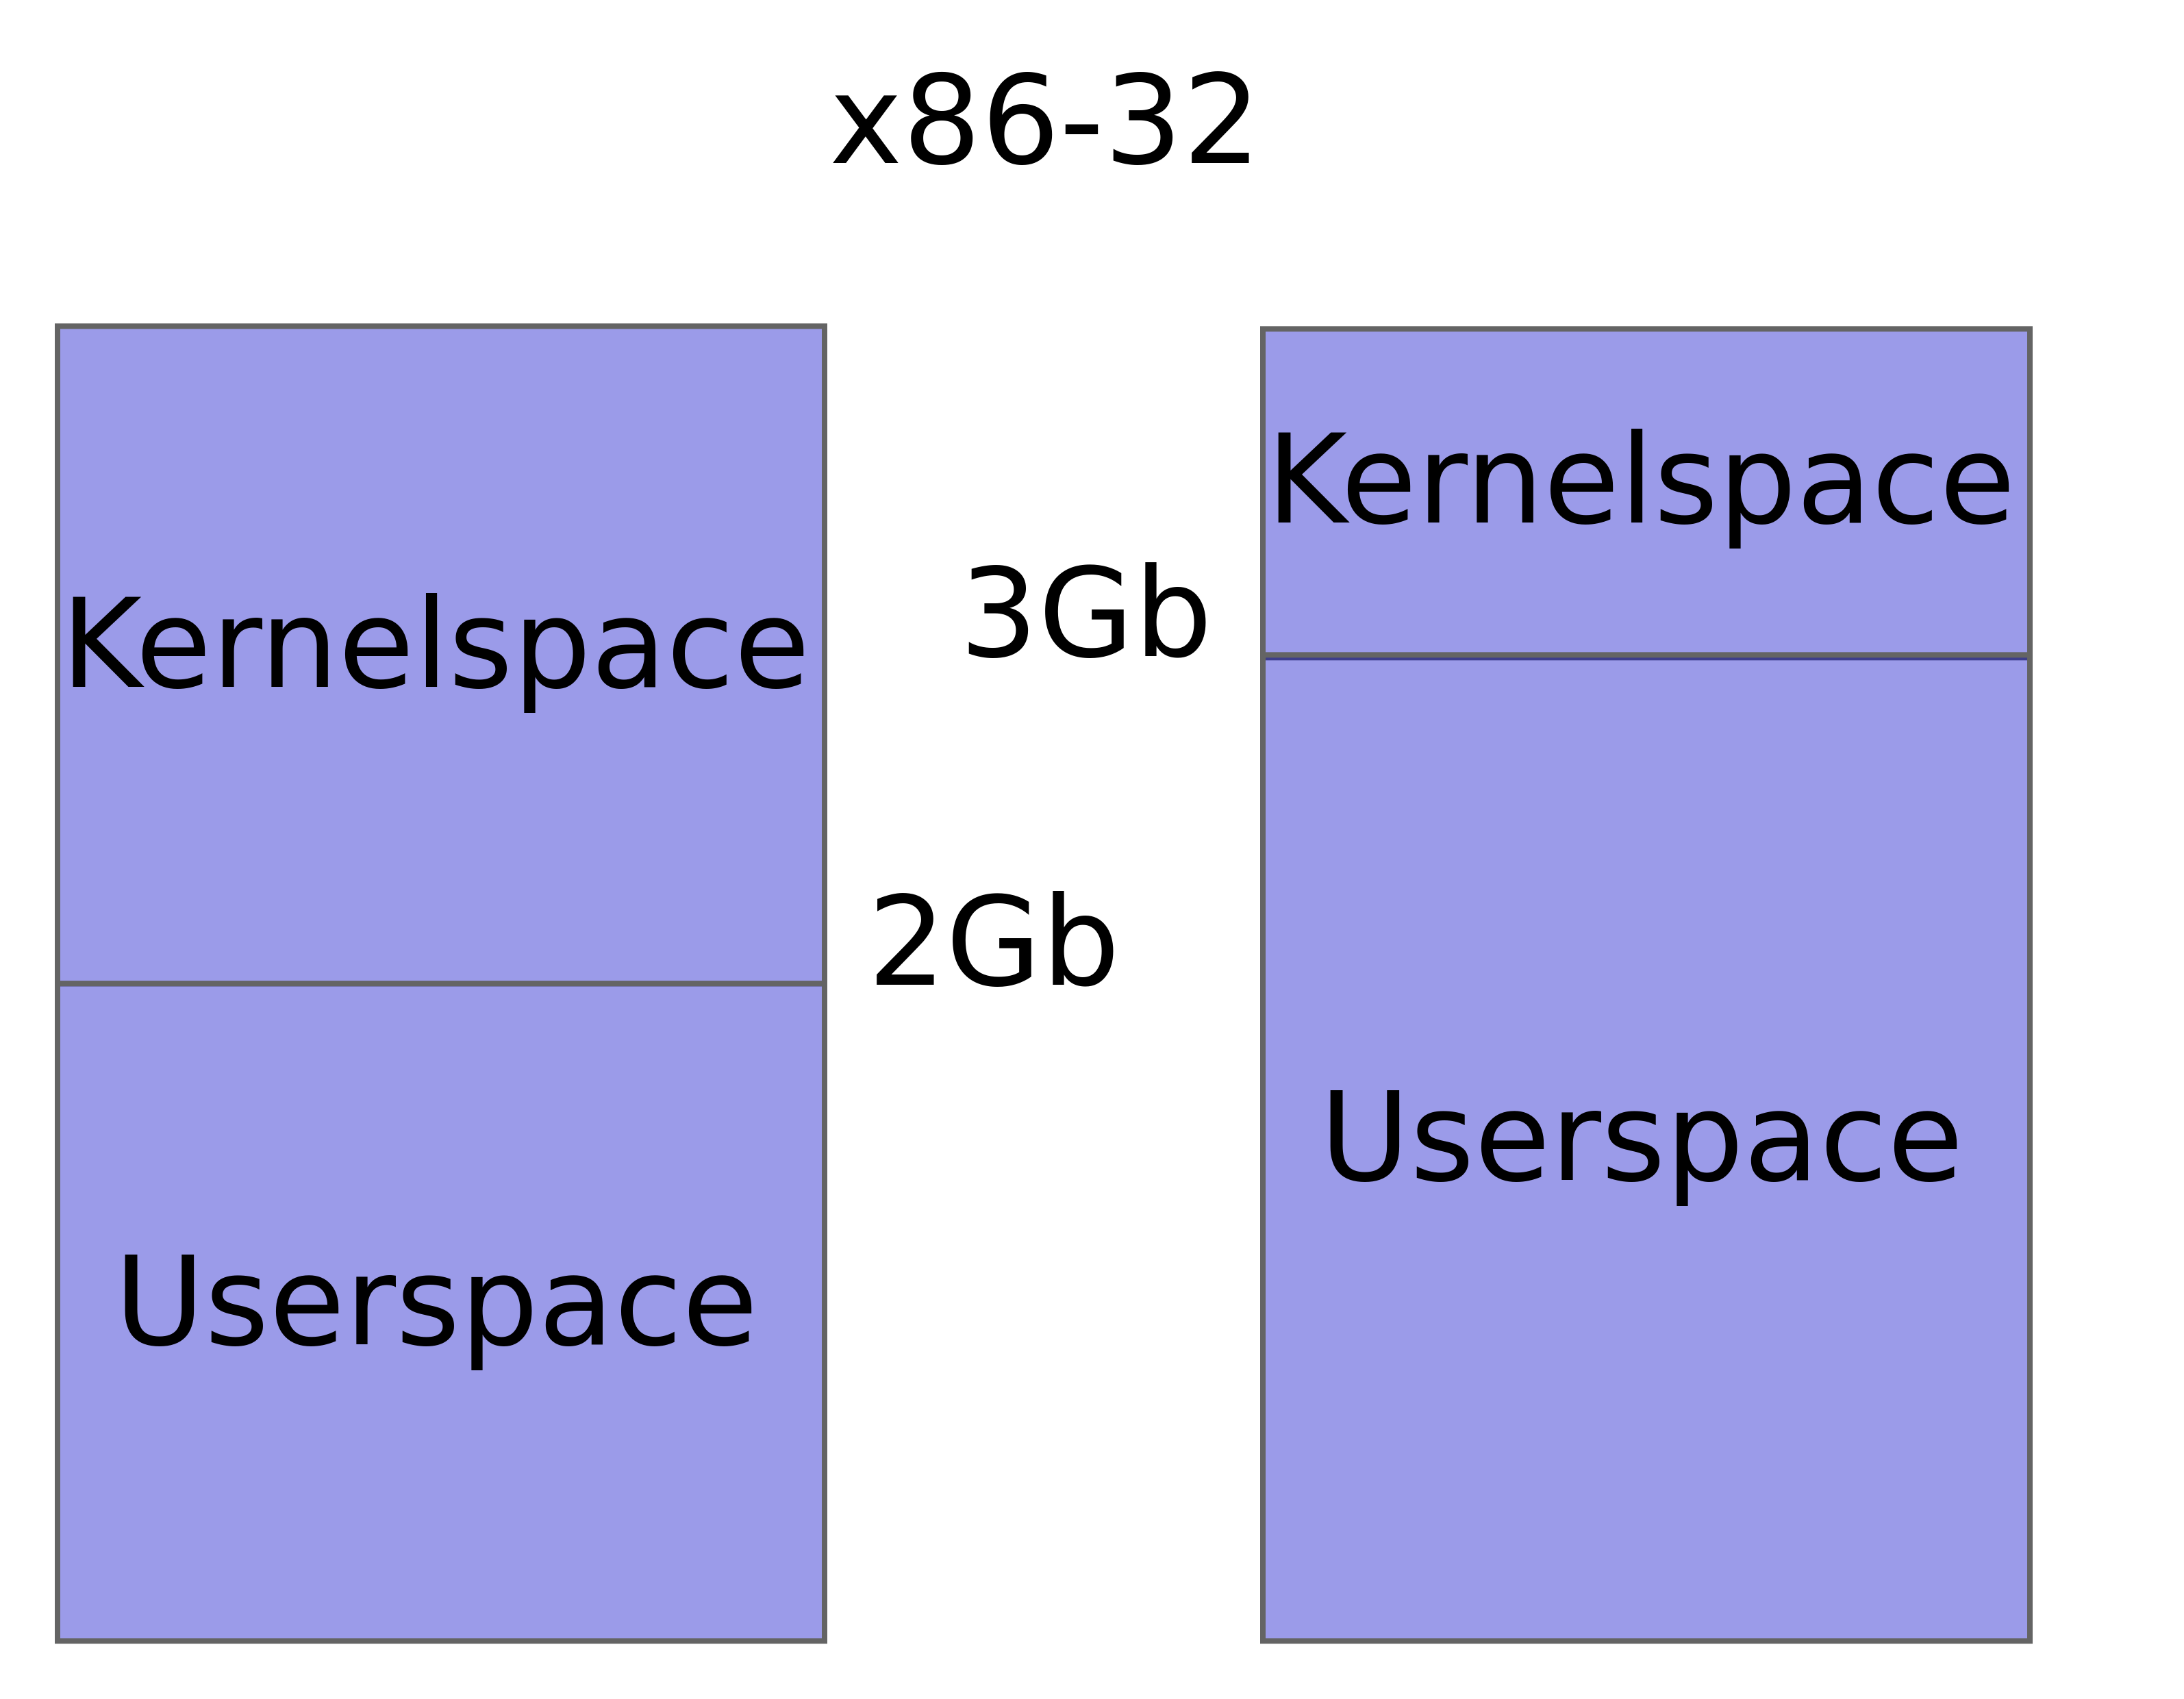
\includegraphics[height=.6\textheight]{x86}
\end{frame}

\begin{frame}
\frametitle{Типичное адресное пространство}
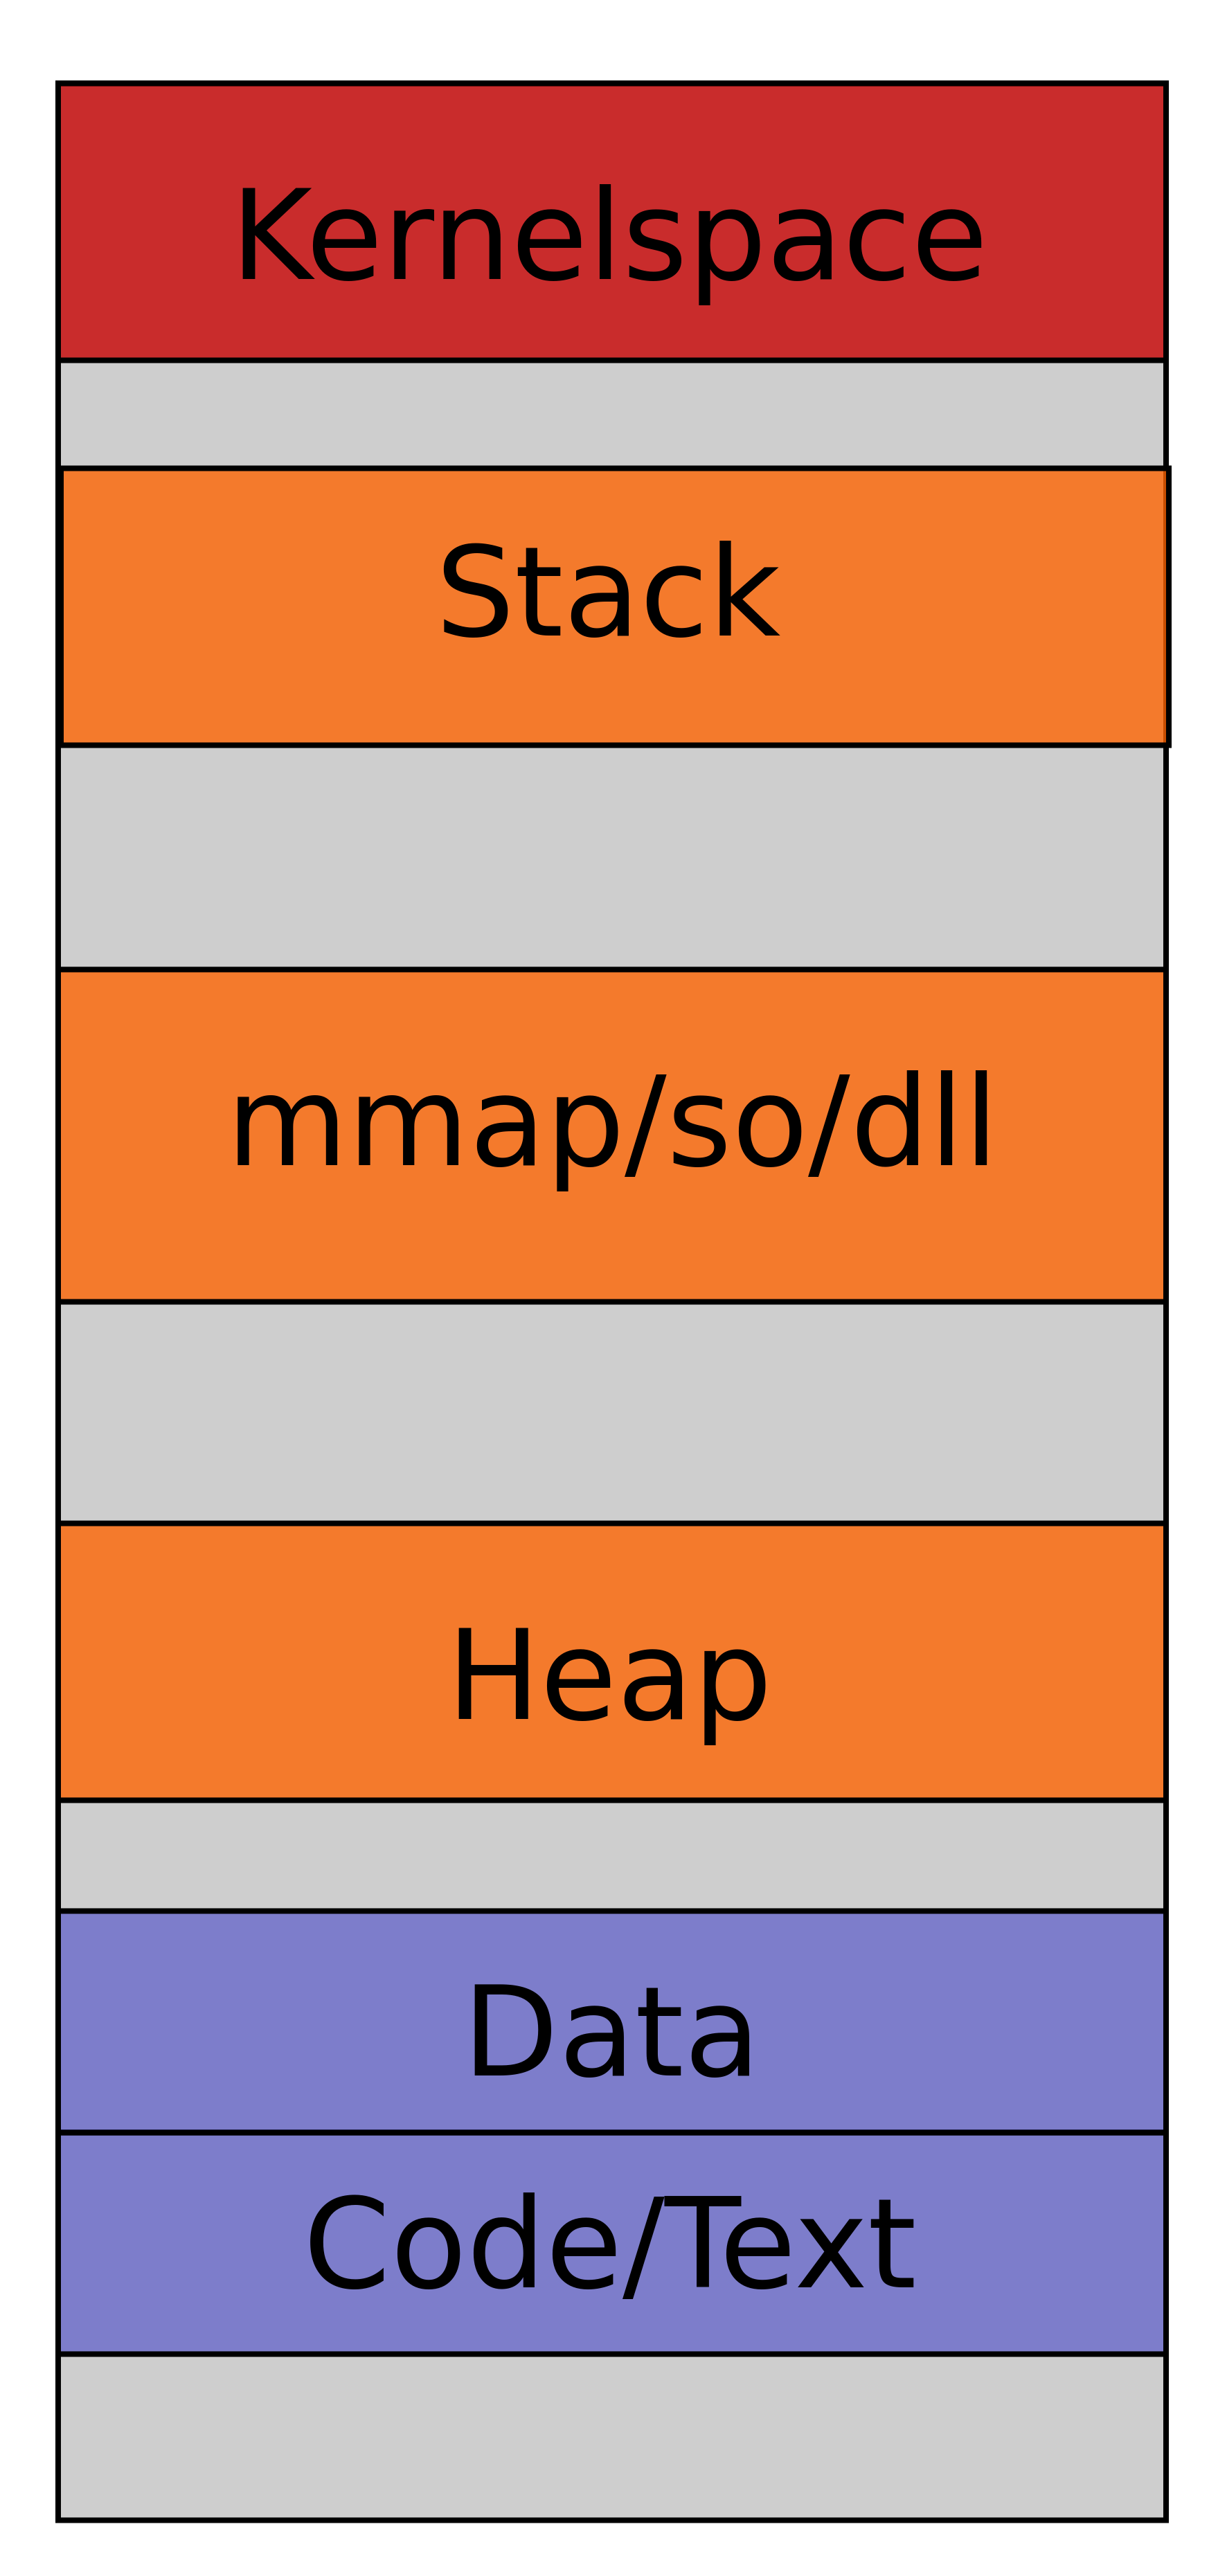
\includegraphics[height=.6\textheight]{address-space}
\end{frame}


\begin{frame}[fragile]
\frametitle{Elf Program Headers}
\begin{lstlisting}
    struct elf64_hdr {
        uint8_t e_ident[16];
        uint16_t e_type;
        uint16_t e_machine;
        uint32_t e_version;
        uint64_t e_entry;

        /* Offset of the program header table */
        uint64_t e_phoff;

        uint64_t e_shoff;
        uint32_t e_flags;
        uint16_t e_ehsize;

        /* The size of a program header table entry */
        uint16_t e_phentsize;
        /* The number of entries in the program
           header table */
        uint16_t e_phnum;

        uint16_t e_shentsize;
        uint16_t e_shnum;
        uint16_t e_shstrndx;
    } __attribute__((packed));
\end{lstlisting}
\end{frame}

\begin{frame}[fragile]
\frametitle{Elf Program Headers}
\begin{lstlisting}
    struct elf64_phdr {
        /* There are different types of segments,
           we need PT_LOAD == 1 */
        uint32_t p_type;

        /* Read/Write/Execute */
        uint32_t p_flags;

        /* Offset of the segment in the file */
        uint64_t p_off;

        /* The logical address of the segment in memory */
        uint64_t p_vaddr;
        uint64_t p_paddr;

        /* The size of the file image of the segment */
        uint64_t p_filesz;

        /* The size of the memory image of the segment */
        uint64_t p_memsz;

        uint64_t p_align;
    } __attribute__((packed));
\end{lstlisting}
\end{frame}

\begin{frame}
\frametitle{Загрузка исполняемого файла}
\begin{itemize}
    \item<1->Подготовить адресное пространство согласно описанию в файле
    \begin{itemize}
        \item<2->аллоцировать память и настроить таблицы страниц;
        \item<3->скопировать код и данные из файла в память;
        \item<4->возможно создать стек отдельно.
    \end{itemize}
    \item<5->"Прыгнуть" в userspace
    \begin{itemize}
        \item<6->передать управление точке входа, указанной в файле;
        \item<7->возможно, понизить уровень привилегий.
    \end{itemize}
\end{itemize}
\end{frame}

